\section{Casi d'uso}

\subsection{Attori}
In un diagramma dei casi d'uso, gli attori rappresentano le entità esterne che interagiscono con il prodotto \textit{Etherless}. Essi si possono distinguere in due categorie:
\begin{itemize}
	\item \textbf{Attori primari:} coinvolti nell'esecuzione dei casi d'uso, interagiscono con il servizio per soddisfare i propri bisogni;
	\item \textbf{Attori secondari:} forniscono servizio o supporto al sistema. 
\end{itemize}
Per l'applicativo non è stato individuato alcun attore secondario, verranno dunque riportati in seguito i soli attori primari.

\subsubsection{Attori primari}
\begin{figure}[h]
	\centering
	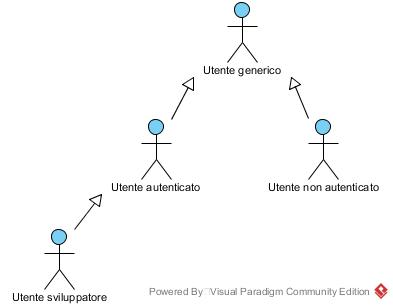
\includegraphics[width=9.7cm]{res/img/gerarchiaAttoriPrimari.jpg}
	\caption{Gerarchia attori primari}
\end{figure}

Sono state identificate quattro diverse tipologie di attori primari relazionati tra loro in maniera gerarchica:

\begin{itemize}
	\item \textbf{Utente generico:} utente che ha eseguito il comando per l'avvio dell'applicativo tramite \textit{Etherlesss-cli};
	\item \textbf{Utente non autenticato:} utente che non ha ancora eseguito l'accesso o la registrazione al network \textit{Ethereum\glo} e che dunque non potrà usufruire delle funzionalità dell'applicazione;
	\item \textbf{Utente autenticato:} utente che ha eseguito l'accesso al network \textit{Ethereum\glo} e che potrà eseguire i comandi messi a disposizione del servizio per gli utenti utilizzatori;
	\item \textbf{Utente sviluppatore:} utente che ha la possibilità di eseguire il deploy di funzioni Javascipt proprie, oltre che eseguire le altre funzioni messe a disposizione dagli altri utenti del servizio.
\end{itemize}



\subsection{Elenco dei casi d'uso}

\begin{figure}[h]
	\centering
	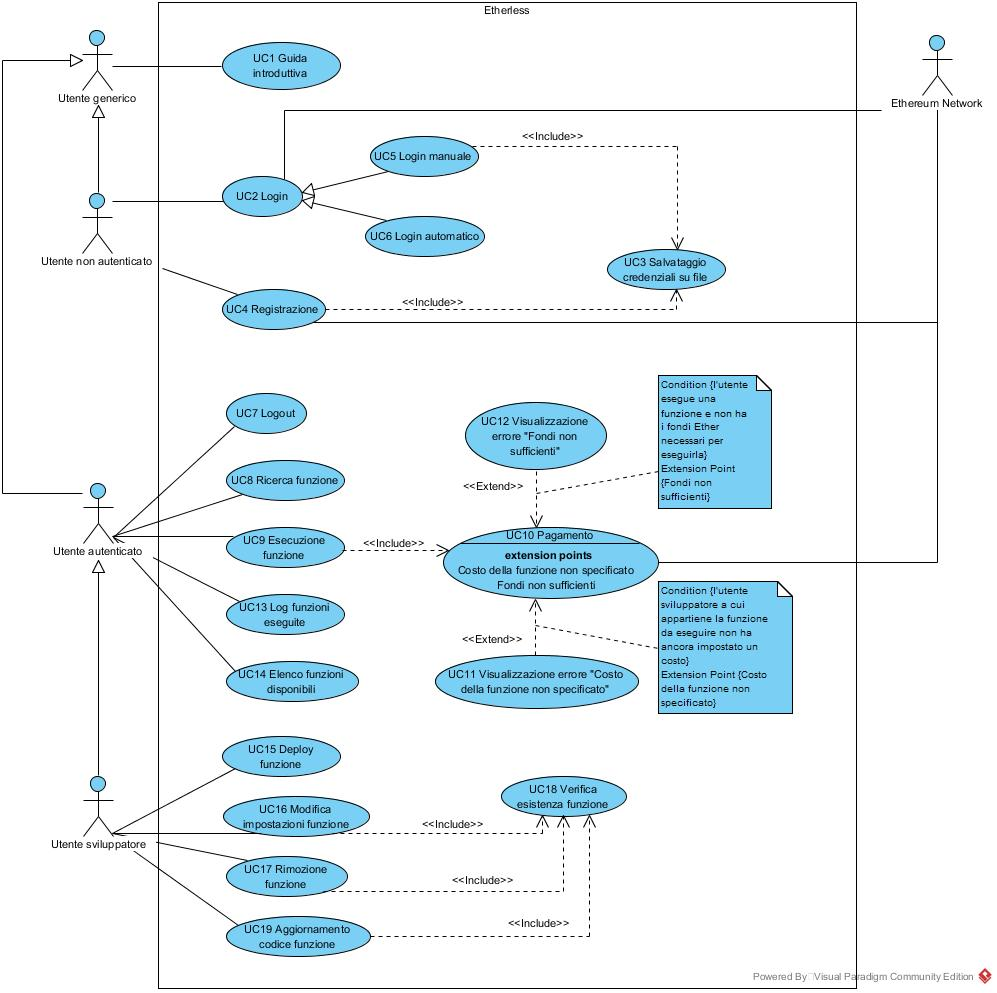
\includegraphics[width=12.3cm]{res/img/useCaseDiagram.jpg}
	\caption{Casi d'uso principali}
\end{figure}
\newpage
\subsubsection{UC1 - Guida introduttiva}
\begin{itemize}
	\item \textbf{Attori primari:} Utente generico;
	\item \textbf{Descrizione:} l'utente generico, appena entrato nell'applicazione, visualizza una guida dei comandi utilizzabili; 
	\item \textbf{Pre-condizioni:} il sistema è raggiungibile e l'applicazione è stata avviata mediante l'apposito comando;
	\item \textbf{Post-condizioni:} Nella \textit{CLI\glo} vengono visualizzati i comandi utilizzabili dall'utente ed una loro descrizione;
	\item \textbf{Scenario principale:} L'utente visualizza la guida introduttiva.
\end{itemize}
\subsubsection{UC2 - Login}
\begin{itemize}
	\item \textbf{Attori primari:} Utente non autenticato;
	\item \textbf{Descrizione:} l'utente ha la possibilità di autenticarsi al network \textit{Ethereum\glo} mediante un address e di una \textit{private key\glos}; 
	\item \textbf{Pre-condizioni:} l'utente ha visualizzato la guida introduttiva e vuole eseguire l'accesso al network \textit{Ethereum};
	\item \textbf{Post-condizioni:} il sistema avrà autenticato o meno l'utente a seconda dei valori di accesso forniti;
	\item \textbf{Scenario principale:} 
	\begin{enumerate}
		\item Vengono inserite le credenziali di accesso (address e \textit{private key\glos}) in maniera manuale o automatica;
		\item L'utente viene autenticato al network \textit{Ethereum\glo} è può usufruire dei comandi messi a disposizione da \textit{Etherless}.
	\end{enumerate}
	\item \textbf{Specializzazioni:}
	\begin{itemize}
		\item \textbf{UC5:} l'utente ha la possibilità di eseguire il login manuale con l'inserimento di address e \textit{private key\glo} da \textit{CLI\glos};
		\item \textbf{UC6:} l'utente verrà automaticamente autenticato dal sistema se presente un file sul proprio dispositivo contenente le credenziali di accesso.  
	\end{itemize}
\end{itemize}
\subsubsection{UC3 - Salvataggio su file}
\begin{itemize}
	\item \textbf{Attori primari:} Utente non autenticato;
	\item \textbf{Descrizione:} quando l'utente compierà per la prima volta l'accesso o si registrerà al network \textit{Ethereum\glo} mediante il sistema, verrà salvato un file sul suo dispositivo contenente le credenziali di accesso utili per i successivi login automatici; 
	\item \textbf{Pre-condizioni:} l'utente si sta autenticando mediante l'apposito comando al network \textit{Ethereum\glos};
	\item \textbf{Post-condizioni:} il sistema avrà salvato un file contenente address e \textit{private key\glo} sul dispositivo;
	\item \textbf{Scenario principale:} 
	\begin{enumerate}
		\item L'utente esegue l'autenticazione manuale o la registrazione mediante i comandi "login"o "signup";
		\item Il sistema salverà le credenziali per i futuri login automatici.
	\end{enumerate}
\end{itemize}
	
\subsection{Tracciamento attori - casi d'uso}	